% !TEX root = ./paper.tex

\subsection{\tcpls Transport Services}

By leveraging \tcpls records and extensions, we can design new modern transport
services atop the combination of \tcp and \tls. In this subsection, we answer our
second research question {\small\textit{RQ2}} by presenting three transport services:
multiplexing, connection migration and multipath. We leverage the \tcpls records
to multiplex concurrent encrypted bytestreams. By extending the \tls handshake, \tcpls
allows joining several \tcp connections to a single \tcpls session to achieve
connection migration and multipath transport.

\subsubsection{Multiplexing}\label{sec:datastreams}
%%%%%%%%%%%%%%%%%%%%%%%%%%%%%%%%%

\begin{figure}
	\centering
	\begin{bytefield}[bitheight=\widthof{aw}]{32}
		\bitbox[]{1}{\small N} & \bitbox[]{9}{} & \bitbox[]{3}{\small N-32} &
		& \bitbox[]{7}{} &
		\bitbox[]{1}{\small 64} & \bitbox[]{9}{} & \bitbox[]{3}{\small 0} \\
		\bitbox{32}{TLS 1.3 AEAD Initial Vector}  \\
		\bitbox[]{12}{+} & \bitbox[]{8}{} & \bitbox[]{12}{$\oplus$} \\
		\bitbox{12}{\tcpls Stream ID} & \bitbox[]{8}{} & \bitbox{12}{Record sequence}
	\end{bytefield}
	\caption{The AEAD IV of \tcpls Streams is derived from \tls 1.3}
	\label{fig:aead-iv}
\end{figure}

Multiplexing is a modern transport service that has been part of recent protocols such
as \sctp, \quic and HTTP/2.0. The latter also proposed multiplexing with an independent
framing system atop the TLS-encrypted TCP bytestream. In our approach, we choose 
to implement multiplexing with \tcpls records. We dedicate a \tcpls record type to
\tcpls stream data. Each stream has a separate cryptographic context which has several
advantages when combined with connection migration and multipath. \todo{state the advantages?}
A \tcpls stream consists of a sequence of \tcpls stream data records encrypted with its cryptographic
context.

One simple way to provide separate cryptographic contexts is to use multiple application-level
keys. But this is known to degrade the security properties proportionally to the number of
additional keys~\cite{chatterjee2011another}. To overcome this, we propose an
Initial Vector (IV) derivation technique from the \tls session secret.
It maintains the IV uniqueness for all streams and related \tcpls records of a \tcpls connection,
which preserves the security of AEAD algorithms.

Figure~\ref{fig:aead-iv} illustrates how the AEAD IV is computed for a 
given \tcpls record of a \tcpls stream. First the left-most bits of the IV derived from the \tls handshake
is summed with the 32-bit \tcpls Stream ID. Then the right-most bits are XORed with the
stream 64-bit record sequence number. Each \tcpls stream has a separate record sequence number space,
which guarantees that the resulting IV is unique for all records of all \tcpls streams.

%The classical solution to support streams in a transport protocol is to assign
%an identifier to each stream and send the data from stream $x$ as a tuple
%$x,seq,data$ where $seq$ is a sequence number. This is the solution chosen by
%\sctp~\cite{rfc4960} and \quic~\cite{draft-ietf-quic-transport}. \tcpls relies
%on cryptographic properties to support several streams.

%\paragraph*{Cryptographic Details and Tricks} In \tcpls, each stream has its own
%cryptographic context. All streams use the same key but derive a specific
%Initial Vector (IV - also called cryptographic nonce) such that nonce-misuse
%cannot happen. Furthermore, \tcpls derives the IV such that the record sequence
%numbers can securely start at $0$ within each stream.
%
%\tcpls uses only one application-level key for $N$ streams, for each direction.
%We selected this approach to avoid security degradation with the usage of
%multiple keys (by a factor $k$ with $k$ keys)~\cite{chatterjee2011another}.

%To enable all stream sequence numbers to start at 0, we rely on some properties
%of the Authenticated Encryption with Associated Data (AEAD) schemes used by \tls
%1.3. To preserve AEAD security, the AEAD nonce used by \tcpls must be of unique
%use when encrypting and decrypting a record. The initial nonce must also be
%unpredictable for an adversary observing the handshake. \tcpls derives it from
%the \tls handshake session secret in a similar fashion to the \tls
%keys~\cite{rfc8446}. The nonce size ranges from $96$ bits to $128$ bits
%depending on the underlying cipher used. In all cases, for a nonce of size $N$
%bits, \tls computes the cryptographic nonce by concatenating the $N-64$ leftmost
%bits with the 64 lower bits XORed with the record's implicit sequence number
%encoded in 64 bits. XORing the lower 64 bits provides more unpredictability to
%the nonce when the same plaintext is encrypted multiple times with the same
%key~\cite{bellare2016multi,hoang2018multi}. This design implies that we give to
%the underlying cipher the 32 upper bits untouched. The resulting value is then
%concatenated with an internal counter in GCM and used as the blocksize-bits (128
%or 256 bits) stream's counter.
%We observe that the leftmost N-64 bits are available to encode a unique stream number. By
%encoding such a unique number in this part of the cryptographic nonce, we enable
%each stream to start its sequence number at 0 while encrypting its records with
%the same key. This observation means that we can create independent
%cryptographic contexts based on a cryptographic nonce's tweak. This implies
%that stream records can be encrypted and decrypted independently of each other,
%with the same key value. This technique maintains AEAD's core assumption
%(uniqueness of nonce), which means that state of art AEAD's security proof
%starting from that assumption applies to our
%design~\cite{chatterjee2011another} and guarantees the security of our scheme.

%\paragraph*{Carrying Multiple Streams over the Same Transport}
%Thanks to those separate cryptographic contexts, \tcpls can perform concurrent
%encryption and decryption between streams while maintaining decryption
%correctness and security, and potentially also use this capability to process
%different streams over different CPU cores.
%Finally, when different streams are carried
%over the same \tcp connection, \tcpls does not explicitely know which stream
%a received record belongs to. To retrieve this information,
%we also
%leverage the AEAD cipher and check the incoming record's authentication tag
%until we find the stream that properly verifies this tag. This operation is
%lightweight: it does not require full decryption of the record because the AEAD
%ciphers used by \tls 1.3 do Encrypt then MAC (and MAC then Decrypt).
%Looking for the right stream that succeeds the tag verification needs to be
%performed once each time the application writes to another stream over the same
%\tcp connection.
%
%Note that, security-wise, each failed decryption is considered a
%forgery attempt. However, we have large limits on the confidentiality and
%integrity with all AEAD ciphers~\cite{luykx2015limits, aeadlimits} before a
%successful forgery may be considered as a non-negligible probability. For
%example, in the case of ChaCha20 + Poly1305, an adversary making $2^{60}$ forgery
%attempts succeeds with probability $2^{-33}$.


\subsubsection{Connection Migration}\label{sec:multipath}

\tcpls allows joining several \tcp connections to an existing \tcpls session.
We leverage this mechanism to implement several multipath transport services
such as connection migration.
Our design is more secure than the subflow joining mechanism of
\mptcp~\cite{raiciu2012hard,hesmans2015smapp,hesmans2016enhanced}.
To secure the association of new \mptcp subflows, peers exchange short keys
inside cleartext \tcp \texttt{Options} during the \tcp handshake~\cite{rfc6824, rfc8684}.
These keys are then used to authenticate the association of subflows.
An attacker that has observed the key exchange during the \tcp handshake can associate
subflows to an existing \mptcp connection~\cite{rfc6181}.


\begin{figure}[!t]
	\centering
	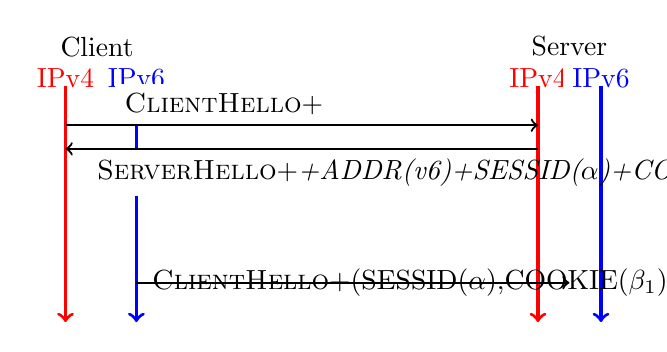
\begin{tikzpicture}
		\colorlet{lightgray}{black!20}
		\tikzstyle{arrow} = [thick,->,>=stealth]
		\tikzset{state/.style={rectangle, dashed, draw, fill=white} }
		\node[black, fill=white] at (0,10) {Client};
		\node[black, fill=white] at (6,10) {Server};
		\node[red, fill=white] at (5.6,9.6) {IPv4};
		\node[blue, fill=white] at (6.4,9.6) {IPv6};
		\node[red, fill=white] at (-0.4,9.6) {IPv4};
		\node[blue, fill=white] at (0.5,9.6) {IPv6};
		\draw[red, very thick,->] (-0.4,9.5) -- (-0.4,6.5);
		\draw[blue, very thick,->] (0.5,9.5) -- (0.5,6.5);
		\draw[red, very thick,->] (5.6,9.5) -- (5.6,6.5);
		\draw[blue, very thick,->] (6.4,9.5) -- (6.4,6.5);
		\draw[black, thick, ->] (-0.4,9) -- (5.6,9) node [midway, fill=white, above,
		text width=4.5cm] {\textsc{ClientHello}+\hello};
		\draw[black, thick, <-] (-0.4,8.7) -- (5.6,8.7) node [pos=0.5, fill=white, below, text width=5.2cm] {\textsc{ServerHello}+\emph{\hello+ADDR(v6)+SESSID($\alpha$)+COOKIE($\beta_1,\beta_2$)}};
		\draw[black, thick, ->] (0.5,7) -- (6.0,7) node [pos=0.4, %fill=white, above,
		text width=4cm] {\textsc{ClientHello}+\join(SESSID($\alpha$),COOKIE($\beta_1$))};
	\end{tikzpicture}
	\caption{\tcpls supports joining additional \tcp
		connections to a \tcpls session. The $SESSID$ and $COOKIE$ in the \textmd{\textsc{ServerHello}} are encrypted with the
		handshake key.}
	\label{fig:join-example}
\end{figure}


\textbf{Joining \tcp connections}. \tcpls leverages its secure records and extensions
to solve this problem in a more secure
manner. Figure~\ref{fig:join-example} illustrates the \tls and \tcpls messages 
exchanged when a client connects to a server over IPv4 and joins another connection
over IPv6.
First, the client sends a \textsc{ClientHello} containing a \hello.
Then, the server replies with a \textsc{ServerHello}
containing three types of encrypted extensions. First, the server announces its IPv6 address.
Second, it associates one identifier $\alpha$ to the \tcpls session in \emph{SESSID($\alpha$)}. 
%It uniquely identifies the \tcpls session on the server. 
Third, the server provides a list
of \tcpls session cookies $\beta_1,\beta_2$ in the \emph{COOKIE} extension.
Each of these session cookies enables the client
to associate one additional \tcp connection to the \tcpls session. Thus by sending $n$
cookies over a session, the server limits the client to associate up to
$n$ \tcp connections. This prevents resource exhaustion attacks
that are difficult to counter with \mptcp. The server can later send additional
cookies and update its list of addresses.

To join a new \tcp connection to the \tcpls session, for instance over IPv6, the client
sends a \textsc{ClientHello} message containing the session identifier
(SESSID($\alpha$) in Fig.~\ref{fig:join-example}) and one of the
cookies provided by the server (COOKIE($\beta_1$) in Fig.~\ref{fig:join-example}). 
The server uses the session identifier $\alpha$ to find the corresponding \tcpls session
and checks the validity of the cookie. If the \tcpls session and cookie are valid, the \tcp
connection is joined to the \tcpls session. The session identifier and
cookie play that same role as the \mptcp token. From a security viewpoint, the \tcpls
session cookie is longer than the \mptcp token, it is sent encrypted
in the initial \textsc{ServerHello} message, and can only be used once.
%(i.e.,
%when the server receives a valid cookie, it accepts the connection, attaches it
%to the right \tcpls session, and discards the cookie).


%\tcpls includes a Connection Manager (CM) that controls the underlying \tcp
%connections.
%The CM is fully configurable and exposed to applications through the \tcpls API.
%\tcpls enables the client or the server to associate new \tcp connections to an
%existing \tcpls session. This is similar to \mptcp's path
%managers~\cite{raiciu2012hard,hesmans2015smapp,hesmans2016enhanced},
%but with some differences. First, \tcpls does not suffer from the same
%security limitations as \mptcp. Second, \tcpls supports several multipathing
%modes, including connection failover, bandwidth aggregation and non-aggregated
%multiple paths.

%\paragraph*{1) Better Security Than \mptcp} A \mptcp connection gathers several
%underlying connections called subflows. To ``secure'' the attachment of
%additional subflows, \mptcp hosts exchange short keys in plaintext inside \tcp
%options during the \tcp handshake~\cite{rfc6824, rfc8684}. These keys are then
%used later to authenticate the attachment of subflows. An
%attacker that has observed the initial handshake can attach any subflow to an
%existing \mptcp connection~\cite{rfc6181}. \tcpls leverages its secure channel
%to solves this \texttt{``connection join''} problem in a more secure
%manner. Consider a client connecting to a dual-stack server
%(Fig.~\ref{fig:join-example} depicts the \tls messages exchanged in such a
%scenario). The client sends a \textsc{ClientHello} containing the \tls
%extension to negotiate \tcpls. The server replies with a \textsc{ServerHello}
%with three types of encrypted extensions. First, the server announces its IPv4
%and IPv6 addresses. Second, it associates one identifier to the \tcpls session
%(SESSID($\alpha$) in Fig.~\ref{fig:join-example}). It uniquely
%identifies the \tcpls session on the server. Third, the server provides a list
%of \tcpls session cookies (COOKIE($\beta_1,\beta_2$) on
%Fig.~\ref{fig:join-example}). Each of these session cookies enables the client
%to attach one additional \tcp connection to the \tcpls session. By sending $n$
%cookies, the server indicates that it currently accepts the attachment of only
%$n$ \tcp connections to this session. This prevents resource exhaustion attacks
%that are difficult to counter with \mptcp. The server can send additional
%cookies later and update its list of addresses.
%
%To attach a new connection, e.g., using the server's IPv6 address, the client
%sends a \textsc{ClientHello} message containing the session identifier
%(SESSID($\alpha$) on Fig.~\ref{fig:join-example}) and one of the server's
%cookies (COOKIE($\beta_1$) on Fig.~\ref{fig:join-example}). The server checks
%the validity of the cookie and then uses the session identifier to attach the
%new \tcp connection to the right \tcpls session. The session identifier and
%cookie play that same role as \mptcp's token. From a security viewpoint, \tcpls'
%session cookie is longer than \mptcp's token. Furthermore, it is sent encrypted
%in the initial \textsc{ServerHello} message, and can only be used once (i.e.,
%when the server receives a valid cookie, it accepts the connection, attaches it
%to the right \tcpls session, and discards the cookie).


\textbf{Passive Connection Migration}. 
Upon network outage, \tcpls leverage its joining mechanism to recover the session
over another \tcp connection. To do achieve it, \tcpls sends stream-level record
acknowledgments for the records that have been received
over each stream. Upon network outage, \tcpls moves the
active streams out of the failed \tcp connection to an active one. Furthermore,
the unacknowledged data records sent over the failed \tcp connection are
transmitted again over a functional one.
%\tcpls' Failover mode is optional. Both peers need to activate it or
%negotiate the feature throught the Secure Control Channel.
We discuss in Section~\ref{sec:perf} measurements quantifying the
performance impact of adding \tcpls record-level acknowledgments. We also give a
trace example involving a file transfer and the failover protocol in
Appendix~\ref{app:failover}.

\textbf{Active Connection Migration}. \tcpls also enables the application
to trigger a connection migration.
%Essentially, it means that \tcpls provides a simple API that enables an
%application to migrate when it wishes to do so (e.g., 
For instance, a smartphone could migrate from LTE to Wi-Fi 
%when the Wi-Fi appears healthy,
and a client using privacy compliant IPv6 addresses~\cite{rfc4941} could restart the underlying \tcp
connection after the expiration of a temporary address. 
%The semantic of
%the application-level connection migration is built from attaching and closing
%streams in the multipath bandwidth aggregation mode. 
%The client that wishes to
%carry such a migration first creates a new \tcp connection and joins the \tcpls
%session over this connection.
To achieve it, the client willing to migrate creates a new \tcp connection and join it to the \tcpls
session. Then, it attaches new streams to the new
connection by sending one \textsc{Stream\_Attach} message per stream that needs
to be migrated. At that moment, the client and the server have potentially
multiple streams opened over the two network paths. Then, after having attached
all its streams to the new path, the migrating host sends a
\textsc{Stream\_Close} message over the old \tcp connection for all old streams.
At this point, the migrating host cannot send new stream data anymore over the
old connection. Once the remote host has received a \textsc{Stream\_Close}
message over the old \tcp connection, it knows that the connection is not
available anymore\todo{?}, and can switch to the other connections. It first sends a
\textsc{Stream\_Close\_Ack} message for each received \textsc{Stream\_Close}.
The migrating host can close the old connection upon reception of the last
\textsc{Stream\_Close\_Ack}, indicating that no more data would be received over
this connection. Note that these messages are \tls records and are thus sent
securely and reliably.% by the underlying \tcp connection.

This second type of migration does not require application-level
acknowledgments, but it cannot survive from one of the
underlying connections' failure. During such a migration, data is sent over two
connections, which brings us to explain how multipath is designed.

\subsubsection{Multipath}

%\paragraph*{3) Different Multipath Modes}
Like \mptcp \cite{raiciu2012hard,rfc6824} or Multipath QUIC \cite{de2017multipath,draft-liu-multipath-quic-02}, \tcpls supports an aggregation mode that maps data over two or more \tcp connections. On multihomed hosts, this can increase the total throughput of a \tcpls session by spreading the data over different network interfaces. In this case, one or more data streams are mapped to two or more underlying \tcp connections and \tcpls schedules different records over different connections.

In addition, \tcpls allows the application to attach its streams to the
underlying \tcp connections in a non-aggrega-ted bandwidth mode. This is a choice left to the application using the API. It has several advantages and drawbacks compared to the aggregation mode. For example, the aggregation mode is simple to use and can potentially saturate the available network paths but can lead to Head-Of-Line (HOL) blocking, since records sent over different \tcp connections need to be eventually re-ordered. The aggregation mode is also more CPU costly, since a zero-copy codepath is technically possible only when the records arrive in order. In the non-aggregated multipath mode, the application needs to take care to fully send an application-level object over the same stream, since the ordering is only guaranteed per-stream in this mode. However, our \tcpls implementation guarantees that this mode will benefit from zero-copy of the decrypted application data, which makes this mode potentially quite interesting for application protocols such as HTTP that need to fetch multiple application objects at the same time.

\subsection{Improving \tcp's Extensibility}

%\label{sec:tcpoptions}
%% Discussing the lack of extensibility of TLS 1.3;
%\begin{figure}[!t]
%  \begin{bytefield}[bitwidth=0.47em]{40}
%    %\bitheader[lsb=0,bitformatting={\tiny\rotatebox[origin=B]{90}}]{0,7,8,15,16,23,24,31,32,39} \\
%    \bitheader[lsb=0,bitformatting={\tiny}]{0,7,15,23,31,39} \\
%    \begin{rightwordgroup}{Header}
%      \bitbox{8}{Type} & \bitbox{16}{Version} & \bitbox{16}{Length}
%    \end{rightwordgroup}\\
%    \begin{rightwordgroup}{Payload}
%      \bitbox{16}{Option Type} & \bitbox{16}{User Timeout} & \bitbox{8}{TType}
%     %&\wordbox[lrb]{1}{Padding... (to match the AEAD block size)}
%    \end{rightwordgroup}\\
%  \end{bytefield}
%  \caption{All \tcpls records have the same type but differ in their encrypted TType. This sample record contains the User Timeout \tcp option.}
%  \label{fig:ex_record}
%\end{figure}

\todo{Move this into the section 2 or intro}
\tcp~\cite{rfc793} limits the size of the entire \tcp header (including options) to 64 bytes. Unfortunately, the \tcp designers did not foresee that many \tcp extensions would be standardized. Today, the \tcp header size becomes a constraint.
%For example, it severely limits the number of gaps that
%can be covered by selective acknowledgments.
The restriction gets more strict with extensions such as \mptcp~\cite{rfc6824} that consume more space in the \tcp header. The IETF has discussed this problem for several years, but the latest attempt to solve it~\cite{draft-ietf-tcpm-tcp-edo-10} has not yet been implemented by major \tcp stacks.
%
%\tcpls provides more space for \tcp options. First, with \tcpls, \tcp
%options can be negotiated during the \tls handshake. Since the \tls messages are
%included in the \tcp payload, there is more space to carry them. Another
%advantage of this approach is that the \tcp options are secured by \tls. This
%implies that they cannot be modified by middleboxes. This could be an advantage,
%but could also prevent \tcpls from correctly working through some types of
%transparent \tcp proxies.
%
%Second, \tcpls can also carry \tcp options inside \tls records. \tcpls includes
%one record type to carry \tcp options. This new type of records can be used to
%carry TCP options that need to be exchanged reliably such as the \tcp User
%Timeout option \cite{rfc5482}, \mptcp's \texttt{ADD\_ADDR} and
%\texttt{REMOVE\_ADDR} option and experimental \tcp options \cite{rfc6994}.

\subsection{Finishing a \tcpls connection}
%%%%%%%%%%%%%%%%%%%%%%%%%%%%%%%%%%%%%%%%
\tcpls's semantic offers a secure stream abstraction to the application.
Streams can be attached to and closed from what we call a \texttt{transportid}
(the application does not have any knowledge of the \tcp interface). When a
stream is attached for the first time to a \tcp connection, this connection
becomes active. The only way to gracefully closes a \tcp connection is by
securely closing all streams attached to it, then \tcpls gracefully closes the
\tcp connection. That is, if \tcpls receives a \rst or a \fin over an active
\tcp connection, it tries to re-establish a \tcp connection. If failover is
enabled, \tcpls tries another network path first. Otherwise, a connection over
the same IP source and destination is reestablished and the streams are moved to
this new \tcp connection. If failover is not enabled, \tcpls would
opportunistically try to reestablish the connection. However, if failover is not
enabled and records were in flight while receiving an illegitimate \rst or \fin
(e.g., sent by a middlebox), \tcpls may suffer from a decryption error, and
report a critical error to the application leading to the termination of the
session.
